%%%%%%%%%%%%%%%%%%%%%%%%%%%%%%%%%%%%%%%%%
% baposter Landscape Poster
% LaTeX Template
% Version 1.0 (11/06/13)
%
% baposter Class Created by:
% Brian Amberg (baposter@brian-amberg.de)
%
% This template has been downloaded from:
% http://www.LaTeXTemplates.com
%
% License:
% CC BY-NC-SA 3.0 (http://creativecommons.org/licenses/by-nc-sa/3.0/)
%
%%%%%%%%%%%%%%%%%%%%%%%%%%%%%%%%%%%%%%%%%

% \title{CSAFE poster template}

%-------------------------------------------------------------------------
%	PACKAGES AND OTHER DOCUMENT CONFIGURATIONS
%-------------------------------------------------------------------------

\documentclass[landscape, a0paper, fontscale=0.275, margin = 30mm]{baposter} % Adjust the font scale/size here
% Other options:
%   - showframe (shows frame around whole poster, useful for debugging
%   - movebody=Xpt (moves body - center on page)
%   - a4shrink (shrink to A4 for handouts)


% \immediate\write18{./convert_tiff_pdf.sh}

%%%%%%%%%%%%%%%%%%%%%%%%%%%%%%%%%%%%%%%%%%%%%%%%%%%%%%%%%%%%%%%%%%%%%%%%%%%%%%%%
%%% Packages that make baposter work well(ish)                               %%%
%%%%%%%%%%%%%%%%%%%%%%%%%%%%%%%%%%%%%%%%%%%%%%%%%%%%%%%%%%%%%%%%%%%%%%%%%%%%%%%%

% This removes any blank page added in the beginning of a document
\usepackage{atbegshi}% http://ctan.org/pkg/atbegshi
\AtBeginDocument{\AtBeginShipoutNext{\AtBeginShipoutDiscard}}
\pretolerance=10000

\usepackage{natbib} % References

\usepackage{setspace}
\usepackage{graphicx} % Required for including images
\usepackage{booktabs} % Top and bottom rules for tables
\usepackage{tabularx} % Stretchy tables
\usepackage{tabu} % Stretchy tables
\usepackage[hypcap=false,font=small,labelfont=bf]{caption} % Required for
                                                           % specifying captions
                                                           % to tables and
                                                           % figures
\usepackage[export]{adjustbox} % Frames around images
\usepackage{url} % Formats URLs properly (hyperref doesn't work with baposter)
\urlstyle{sf}

% \usepackage{tikz} % Required for flow chart
% \usetikzlibrary{shapes,arrows} % Tikz libraries required for the flow chart
%                                % in the template

\usepackage{multicol} % Required for multiple columns
\setlength{\columnsep}{1.5em} % Slightly increase the space between columns
\setlength{\columnseprule}{0mm} % No horizontal rule between columns

\usepackage{enumitem} % Itemize separation
\setlist{nosep} % or \setlist{noitemsep} to leave space around whole list
\setitemize{nolistsep,leftmargin=*}
\setenumerate{nolistsep,leftmargin=*}
\newcommand{\compresslist}{
% Define a command to reduce spacing within itemize/enumerate environments,
% this is used right after \begin{itemize} or \begin{enumerate}
\setlength{\itemsep}{1pt}
\setlength{\parskip}{0pt}
\setlength{\parsep}{0pt}
}

\usepackage{amsmath} % For typesetting math
\usepackage{amssymb} % Adds new symbols to be used in math mode
\usepackage{fontspec} % Use fonts

% This command allows you to set the border/header color in one go
\newcommand{\headercolorbox}[4]{%
  \begin{posterbox}[#3,borderColor=#2,headerColorOne=#2,headerColorTwo=#2]{#1}
    #4
  \end{posterbox}
}
%%%%%%%%%%%%%%%%%%%%%%%%%%%%%%%%%%%%%%%%%%%%%%%%%%%%%%%%%%%%%%%%%%%%%%%%%%%%%%%%

%%%%%%%%%%%%%%%%%%%%%%%%%%%%%%%%%%%%%%%%%%%%%%%%%%%%%%%%%%%%%%%%%%%%%%%%%%%%%%%%
%%% CSAFE Styling (from Identity Guide)                                      %%%
%%%%%%%%%%%%%%%%%%%%%%%%%%%%%%%%%%%%%%%%%%%%%%%%%%%%%%%%%%%%%%%%%%%%%%%%%%%%%%%%
\setmainfont[Ligatures=TeX]{Sanchez}[
  Path=fonts/, Extension = .ttf,
  UprightFont=*-Regular,
  ItalicFont=*-Italic]
\setsansfont[Ligatures=TeX]{Montserrat}[
  Path=fonts/, Extension = .ttf,
  UprightFont=*-Light,
  BoldFont=*-Bold,
  ItalicFont=*-LightItalic,
  BoldItalicFont=*-BoldItalic]
\setmonofont[Ligatures=TeX]{Inconsolata}[
  Path=fonts/, Extension = .ttf,
  UprightFont=*-Regular,
  BoldFont=*-Bold]
% Use montserrat as default font
\renewcommand{\familydefault}{\sfdefault}
% Create command \sanchez to use for headings with Sanchez
\newfontfamily\sanchez{Sanchez}

\definecolor{white}{rgb}{1,1,1} % Defines the color used for content box headers
% CSAFE Colors
\definecolor{csafedarkblue}{rgb}{0,.227,0.439} % Default for content box headers
\definecolor{csafelightblue}{rgb}{.251, .706, .898}
\definecolor{csafegreen}{rgb}{.467, .737, .122}
\definecolor{csafered}{rgb}{.811, .039, .173}
\definecolor{csafegrey}{rgb}{.541, .541, .553}
\definecolor{csafegray}{rgb}{.541, .541, .553}

\renewcommand{\figurename}{Fig.} % Shorten figure caption label
\graphicspath{{figures/}{images/}{figure/}{image/}} % Directory in which figures are stored

\newcommand\csafelogo[1][height=7em]{
\includegraphics[#1]{figures/logo.png}}
\newcommand\nistlogo[1][height=5em]{
\includegraphics[#1]{figures/logo-NIST.jpg}}

\newcommand\csafeboilerplate{\vspace*{0.05em}\hspace{-5mm}\tiny{This work was partially funded by CSAFE through Cooperative Agreement \# 70NANB15H176 between NIST and Iowa State University, which includes activities carried out at Carnegie Mellon University, University of California Irvine, and University of Virginia}}

%%%%%%%%%%%%%%%%%%%%%%%%%%%%%%%%%%%%%%%%%%%%%%%%%%%%%%%%%%%%%%%%%%%%%%%%%%%%%%%%

\graphicspath{{figures/}{DLData/}} % Directory in which figures are stored

\begin{document}
\begin{poster}
{
% grid=true, % show grid to help align stuff
columns=3,
background=none,
colspacing=1em, % Column spacing
textborder=rectangle, % Format of the border around content boxes, can be:
                      % none, bars, coils, triangles, rectangle, rounded,
                      % roundedsmall, roundedright, roundedleft, or faded
boxshade=none,
borderColor=csafedarkblue,
headerheight=0.14\textheight, % Height of the header
headerborder=closed, % Adds a border around the header of content boxes
headershape=rectangle, % Corner in the content box headers, can be: rectangle,
                       % small-rounded, roundedright, roundedleft or rounded
headershade=plain,
headerColorOne=csafedarkblue,
headerColorTwo=csafedarkblue,
headerFontColor=white,
headerfont=\Large\bf, % Large, bold font in the headers of content boxes
linewidth=1.5pt % Width of the border lines around content boxes
}
%-------------------------------------------------------------------------------
%	TITLE SECTION
%-------------------------------------------------------------------------------
%
\csafelogo
{\huge\bf A Longitudinal Database of Athletic Shoe Outsole Wear\vspace{0.3em}} % Poster title
{{\Large Susan VanderPlas, Guillermo Basulto-Elias, James E. Kruse, \\Stacy Renfro, Alicia Carriquiry, Iowa State University}\vspace*{-0.6em}} % Author names and institution
\nistlogo

%---------------------------------------------------------------------------------
%	Study Design
%---------------------------------------------------------------------------------

\headercolorbox{Study Design}{csafelightblue}{name=objectives,column=0,row=0}{
{\bf Shoes}
\begin{itemize}
\item 160 pairs
\item Models: Adidas Seeley, Nike Winflo
\item 2 sizes each in Men and Women's shoes
\item Worn for a minimum of 10,000 steps per week
\item Returned every 5 weeks for assessment\\Initial collection + 3 wear assessments
\end{itemize}
\vspace{.5em}
{\bf Methods}
\begin{enumerate}
\item Pressure Scanner {\small(initial visit, barefoot \& with shoes)}
\item 2D Digital Scanner
\item 3D Laser Scanner
\item Digital Camera
\item Film and Powder Prints
\item Paper and Powder Prints
\item Simulated Crime Scene Style Prints
\end{enumerate}
\vspace{.5em}
{\bf Data Collection Procedures:}
Documentation at \\{\small\url{https://github.com/CSAFE-ISU/Longitudinal_Shoe_Study}}
}

%---------------------------------------------------------------------------------
%	Data Collection Methods
%---------------------------------------------------------------------------------

\headerbox{Data Collection Methods}{name=datacollection,column=0,below=objectives,above=bottom}{
\begin{minipage}[b]{.49\textwidth}
\centering
\includegraphics[width=4.8cm]{DLData/paper_powder_007961L_20180411_6_1_1_kruse_zwart_Kruse}
\captionof{figure}{Paper + Powder Print}
\end{minipage}
\begin{minipage}[b]{.49\textwidth}
\centering
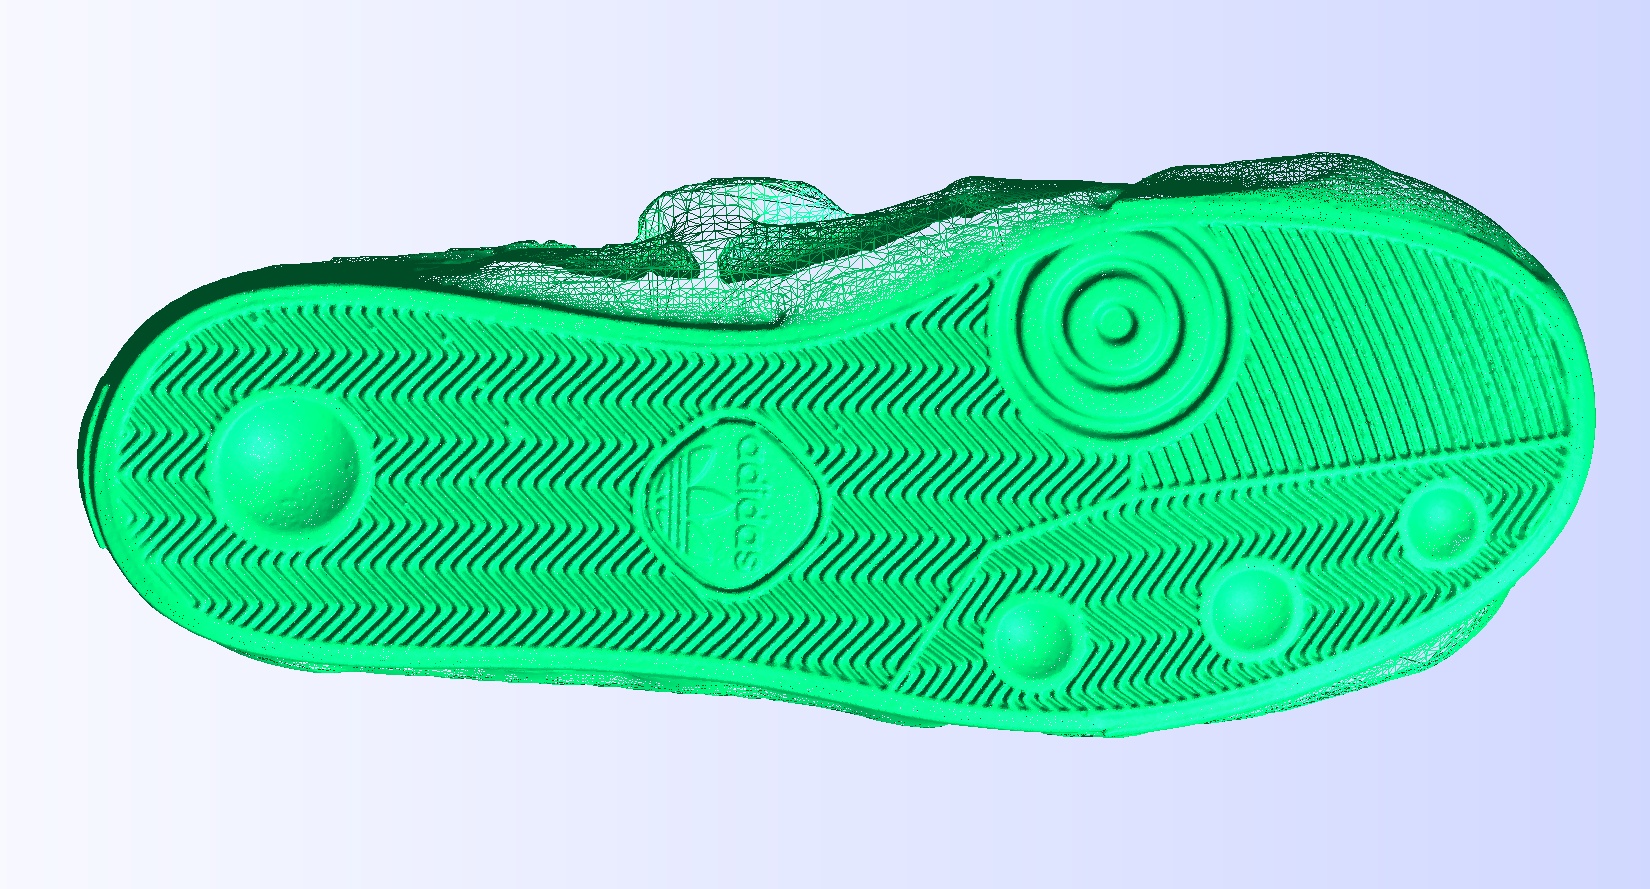
\includegraphics[width=4.8cm]{DLData/stl_render_007961L_20180411_3_2_2_jekruse}
\captionof{figure}{Rendered 3D Scan}
\end{minipage}
\vspace{2em}\\
\begin{minipage}[b]{.49\textwidth}
\centering
\includegraphics[width=4.8cm]{DLData/crime_scene_007961L_20180411_7_1_1_kruse_zwart}
\captionof{figure}{Crime Scene Print}
\end{minipage}
\begin{minipage}[b]{.49\textwidth}
\centering
\includegraphics[width=4.8cm]{DLData/camera_image_007961L_20180411_4_1_1_csafe_jekruse.pdf}
\captionof{figure}{Digital Camera}
\end{minipage}
}

%----------------------------------------------------------------------------------------
%	URL
%----------------------------------------------------------------------------------------

\headercolorbox{Access the Database}{csafered}{name=url,column=1,row=0,span=2}{
\begin{minipage}[c]{.99\textwidth}
\centering
\bf\large\url{https://data.csafe.iastate.edu/LongitudinalShoeStudy/}
\end{minipage}\vspace{-.5em}
}


%----------------------------------------------------------------------------------------
%	Longitudinal Shoe Wear - Nike
%----------------------------------------------------------------------------------------

\headerbox{Nike Winflo - Film Prints}{name=lswn,column=1,below=url}{
\begin{minipage}{\textwidth}
\centering
\begin{tabu} to \textwidth {X[c]X[c]X[c]X[c]}
\includegraphics[height=4.25cm,cframe=csafered]{043758L_20180109_5_1_1_csafe_kruse-basulto-elias-kruse.pdf} &
\includegraphics[height=4.25cm,cframe=csafered]{043758L_20180131_5_1_1_csafe_boekhoff_kruse_zwart.pdf} &
\includegraphics[height=4.25cm,cframe=csafered]{043758L_20180307_5_2_1_basulto_silerio_jekruse.pdf} &
\includegraphics[height=4.25cm,cframe=csafered]{043758L_20180411_5_1_1_bryson_kruse_kruse.pdf}\\
0 steps & 80035 steps & 146844 steps & 255499 steps
\end{tabu}
\end{minipage}
}

%----------------------------------------------------------------------------------------
%	DB Features
%----------------------------------------------------------------------------------------

\headercolorbox{Database Features}{csafegreen}{name=sets,column=1,below=lswn,above=bottom}{
Metadata about the images, shoes, and participants is included in the downloaded zip file.\\
\vspace{.25em}
\begin{minipage}{\textwidth}\centering
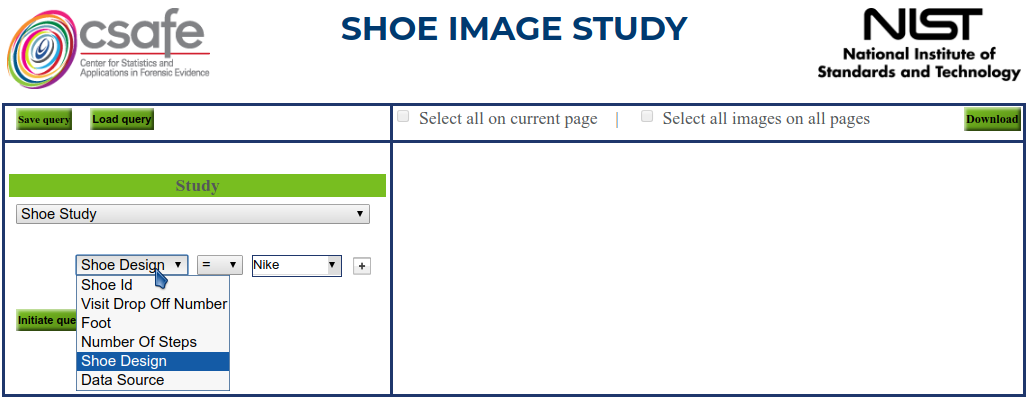
\includegraphics[width=.9\textwidth]{QueryFields.png}\vspace{-.5em}
\captionof{figure}[Query Fields]{6 searchable fields, including design, individual shoe ID, foot, capture method, and number of steps.}
\end{minipage}\vspace{.5em}
\begin{minipage}{\textwidth}\centering
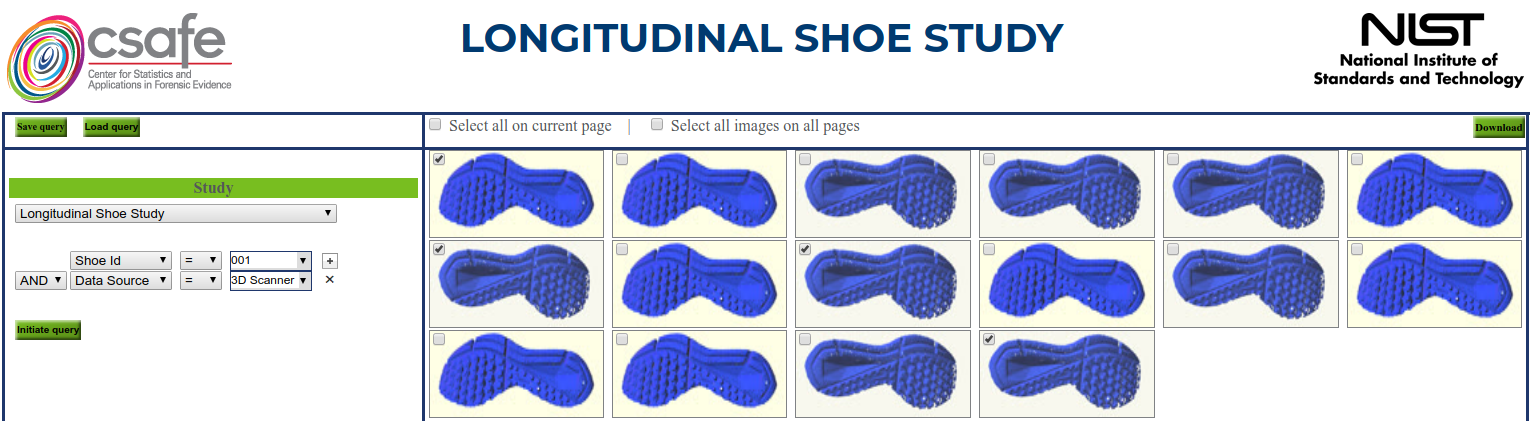
\includegraphics[width=.9\textwidth]{DownloadSelect.png}\vspace{-.5em}
\captionof{figure}{Download only the images you need.}
\end{minipage}\vspace{.5em}
\begin{minipage}{\textwidth}\centering

\includegraphics[width=.5\textwidth]{SaveAndLoad.png}\vspace{-.5em}
\captionof{figure}{Export queries for later.}
\end{minipage}
}

%----------------------------------------------------------------------------------------
%	Longitudinal Shoe Wear - Adidas
%----------------------------------------------------------------------------------------

\headerbox{Adidas Seeley - 2D Digital Scan}{name=lswa,column=2,span=1,below=url}{
\begin{minipage}{.98\textwidth}
\centering
\begin{tabu} to \textwidth {X[c]X[c]X[c]X[c]}
\includegraphics[height=4.25cm]{007961L_20171031_2_1_1_csafe_bpbryson.pdf} &
\includegraphics[height=4.25cm]{007961L_20180124_2_1_1_csafe_bryson.pdf} &
\includegraphics[height=4.25cm]{007961L_20180228_2_1_1_csafe_jekruse.pdf} &
\includegraphics[height=4.25cm]{007961L_20180411_2_1_1_csafe_jekruse.pdf}\\
0 steps & 98753 steps & 129205 steps & 183958 steps
\end{tabu}
\end{minipage}
}



%----------------------------------------------------------------------------------------
%	Build A Query
%----------------------------------------------------------------------------------------

\headercolorbox{Build A Query}{csafegreen}{name=baq,column=2,below=lswa}{
\begin{minipage}{.5\textwidth}\begin{enumerate}\compresslist\small
\item Add new conditions using the $+$ sign
\item Select the join operation to use (AND/OR)\\
{\footnotesize OR joins linked AND queries}
\item Select the filter variable
\item Select the desired value
\item Submit (Initiate Query)
\item Select images for download (right pane)
\end{enumerate}

\end{minipage}\hfill
\begin{minipage}{.475\textwidth}\centering
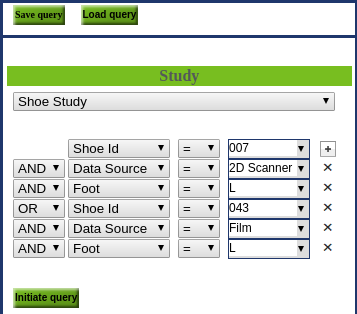
\includegraphics[width=.9\textwidth]{QueryBuilder.png}
\end{minipage}


}

%----------------------------------------------------------------------------------------
%	Other
%----------------------------------------------------------------------------------------

\headercolorbox{Goals}{csafelightblue}{name=goals,column=2,span=1,below=baq,above=bottom}{
The goal of this database is to enable comparisons of wear and individual characteristics, as measured by several different collection methods.

\begin{itemize}\setlength\itemsep{3pt}
\item Compare data acquisition methods
\item Examine individual wear patterns
\item Explore evolution of acquired defects over time
\item Compare wear/defect frequency between shoe models
\end{itemize}
}
\end{poster}
\csafeboilerplate
\end{document}
